\chapter{Referencial Teórico}\label{cp:refteory}
\ABNTEXchapterfont
% Justificativa das tecnologias, comparação 
%Este capítulo é um componente importante para esse estudo, pois fornece uma base  explorando as principais teorias, conceitos e definições existentes sobre as áreas de conhecimento que motivaram a elaboração deste projeto de pesquisa e que guiarão a execução do percurso metodológico.

%Escreva sobre o referencial teórico do seu trabalho

% Qual é o tipo de problema
% Utilizando o artigo do 3DPlanNet
O desenho arquitetônico  contém vários tipos de objetos: paredes, portas, janelas, quartos, nome do cômodo, móveis, as suas dimensões,  entre outros% , e essas informações serão compreendidas pelo computador. 
, essas características dão ao leitor os meios para poder reproduzir o que está no papel no mundo real, nas construções. A transferência do desenho arquitetônico para o a construção é algo estático e não pode ser alterado, gerando um problema se for necessário fazer uma reforma, onde não é mais possível utilizar a mesma planta baixa para gerar um resultado diferente, é então necessário a utilização de um ambiente em que seja possível alterar a organização dos objetos na planta, e isso é possível no ambiente virtual \cite{lv2021residential}.

Caso não tenha o modelo virtual do desenho arquitetônico será necessário fazer a sua reconstrução, o documento será digitalizado depois será processado e para gerar uma estrutura de dados que seja capaz de manipular, no caso desse projeto os dados serão transformados em um modelo 3D.

O processamento da imagem gera alguns problemas sendo solucionados por algoritmos heurísticos, mas atualmente as soluções usam técnicas de aprendizagem profunda \iffalse referênciar? \fi e essa mudança mostrou uma melhora na acurácia na detecção dos objetos \cite{3dplanet2021}.

Um dos problemas que isso gera é a necessidade da criação de datasets devidamente anotados para treinar os modelos de aprendizagem profundas.

A técnica de \cite{3dplanet2021} se mostra interessante por conseguir com 30 imagens anotadas gerar um modelo que \cite{kratochvila2024multi} diz é uma das técnicas de estado da arte.

% Ajudar com base na literatura que ainda existe na 

% Utilizar o resumo/conclusão de cada artigo, e discutir sobre os métodos e os achados e comentar sobre os artigos mostrando que ainda há algo a ser feito 

% Como as pessoas estão resolvendo os problemas
% sugestão de tabelinha de como comparar as diferentes soluções ajuda consideravelmente no entendimento do trabalho



% Motivo de não usar LiDAR: \citeonline{yang2022automated}

% \section{Figuras no texto}\label{cp:refteory:figuras}

% Meu texto a \autoref{figs/batepapo} mostra... figura \ref{figs/batepapo}

% \begin{figure}[H]
%     \centering
%     \caption{Comunicação Interativa entre Usuários.}
%     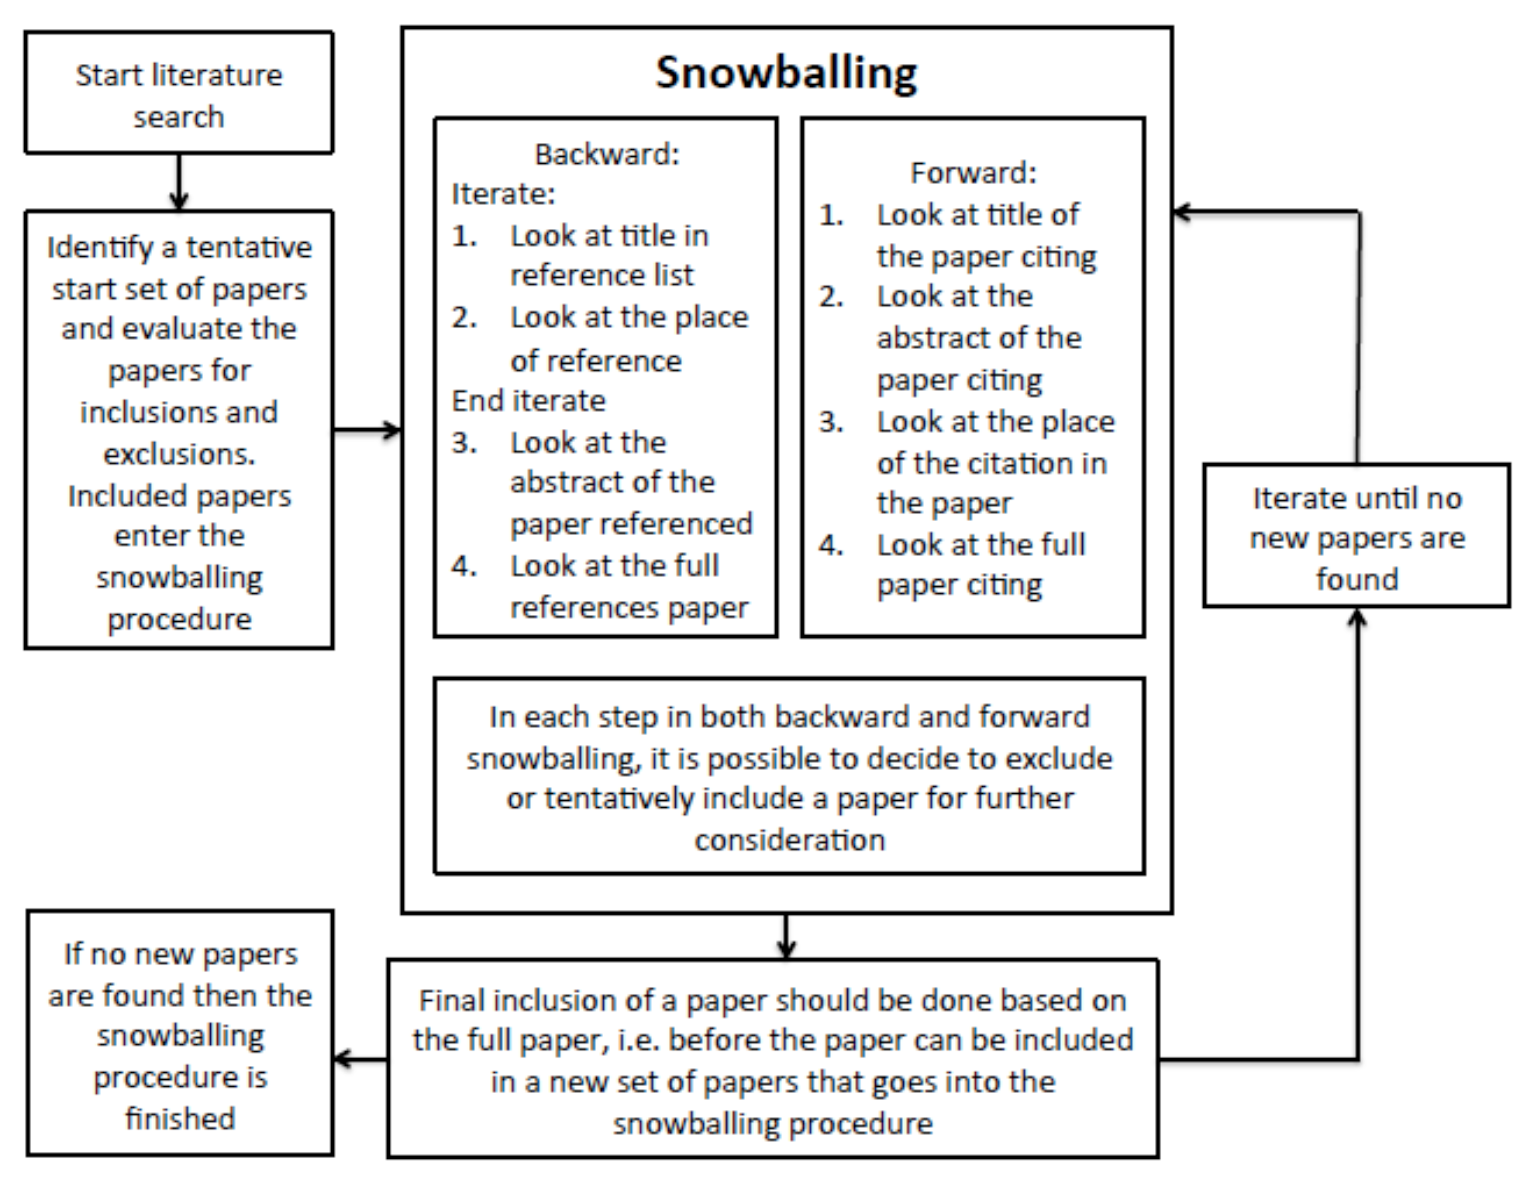
\includegraphics[width=16cm, height=12cm]{imagens/snowballing.png}
%     \legend{Fonte: \citeonline{snowballing4guidelines}.}
%     \label{figs/batepapo}  % Adicionando o label para a figura
% \end{figure}

\section{Considerações Finais}
Se necessário escreva consideracoes finais e faça o link com o que será visto no proximo capítulo
